
\documentclass{article} % For LaTeX2e
\usepackage{iclr2026_conference,times}

\usepackage{booktabs}    % \toprule, \midrule, \bottomrule in tables
\usepackage{enumitem}    % [nosep, leftmargin=1.5em] on itemize
\usepackage{graphicx}    % \includegraphics
\usepackage{amsmath}     % \text inside math, equation environment
\usepackage{hyperref}    % \url, \href
\usepackage[capitalize,noabbrev]{cleveref}  % \cref

% Optional math commands from https://github.com/goodfeli/dlbook_notation.
\input{math_commands.tex}

\usepackage{hyperref}
\usepackage{url}

\title{Disentangled Models Achieve Better Retain--Forget Trade-offs}

\author{Evžen Wybitul \\
  University of Oxford \\
  \And
  Tim G. J. Rudner \\
  University of Toronto \\
  \And
  Christian Schroeder de Witt \\
  University of Oxford
}

\newcommand{\fix}{\marginpar{FIX}}
\newcommand{\new}{\marginpar{NEW}}

\iclrfinalcopy % Uncomment for camera-ready version, but NOT for submission.
\begin{document}

\maketitle

% \begin{abstract}
% \end{abstract}

\section{Introduction}

When knowledge that should be unlearned and knowledge that should be retained share processing pathways, representations, or parameters --- when the two domains are \emph{entangled} in the model --- removing one without damaging the other should intuitively be harder for unlearning methods.
This idea is widespread in the unlearning literature~\citep{barez2025openproblemsmachineunlearning}, but direct experimental evidence for it has been limited.

Unlearning depends on (at least) three factors: the choice of forget and retain datasets, the model being unlearned, and the unlearning algorithm.
Perhaps the most natural test of whether entanglement affects unlearning would hold the datasets and the algorithm fixed and vary only the degree of entanglement in the model.
This has not historically been the approach taken, likely because it was difficult to construct a suite of models with varying levels of entanglement.

Instead, prior work has explored the other two axes.
In image classifier unlearning, \citet{zhao2024what} hold the model and algorithm fixed and vary which examples constitute the forget and retain sets, showing that more entangled datasets are harder to unlearn.
In language model unlearning, the typical approach is to hold the model and datasets fixed and propose a new unlearning algorithm that (at least intuitively) reduces the impact of entanglement and compare it against existing methods~\citep{tang2026logitslatentscontrastiverepresentation, chen2026clue}.
While both lines of work are suggestive, neither isolates the effect of model-level entanglement from other factors.

Our main contribution is to fill this gap --- we hold the algorithm and datasets fixed, and vary the model's entanglement.
We train a suite of six 254M language models on English Wikipedia in which the knowledge of biology is increasingly disentangled from other knowledge using an improved variant of gradient routing~\citep{shilov2025datafilteringknowledgelocalization, cloud2024gradientroutingmaskinggradients}.
On each model in the suite, we measure the retain--forget trade-off of three common unlearning methods: Weighted Gradient Ascent (WGA)~\citep{wang2025rethinking}, Weight Divergence Regularization (WDR)~\citep{siddiqui2025dormant}, and RMU~\citep{li2024wmdp}.
\textbf{We find that more disentangled models consistently achieve better retain--forget trade-offs (\cref{figure:unlearning}):} at a fixed level of forgetting, the most disentangled model incurs roughly $4\times$ lower retain cost than the most entangled model in WGA and RMU, and $1.3\times$ lower in WDR.

\begin{figure}[h]
  \centering
  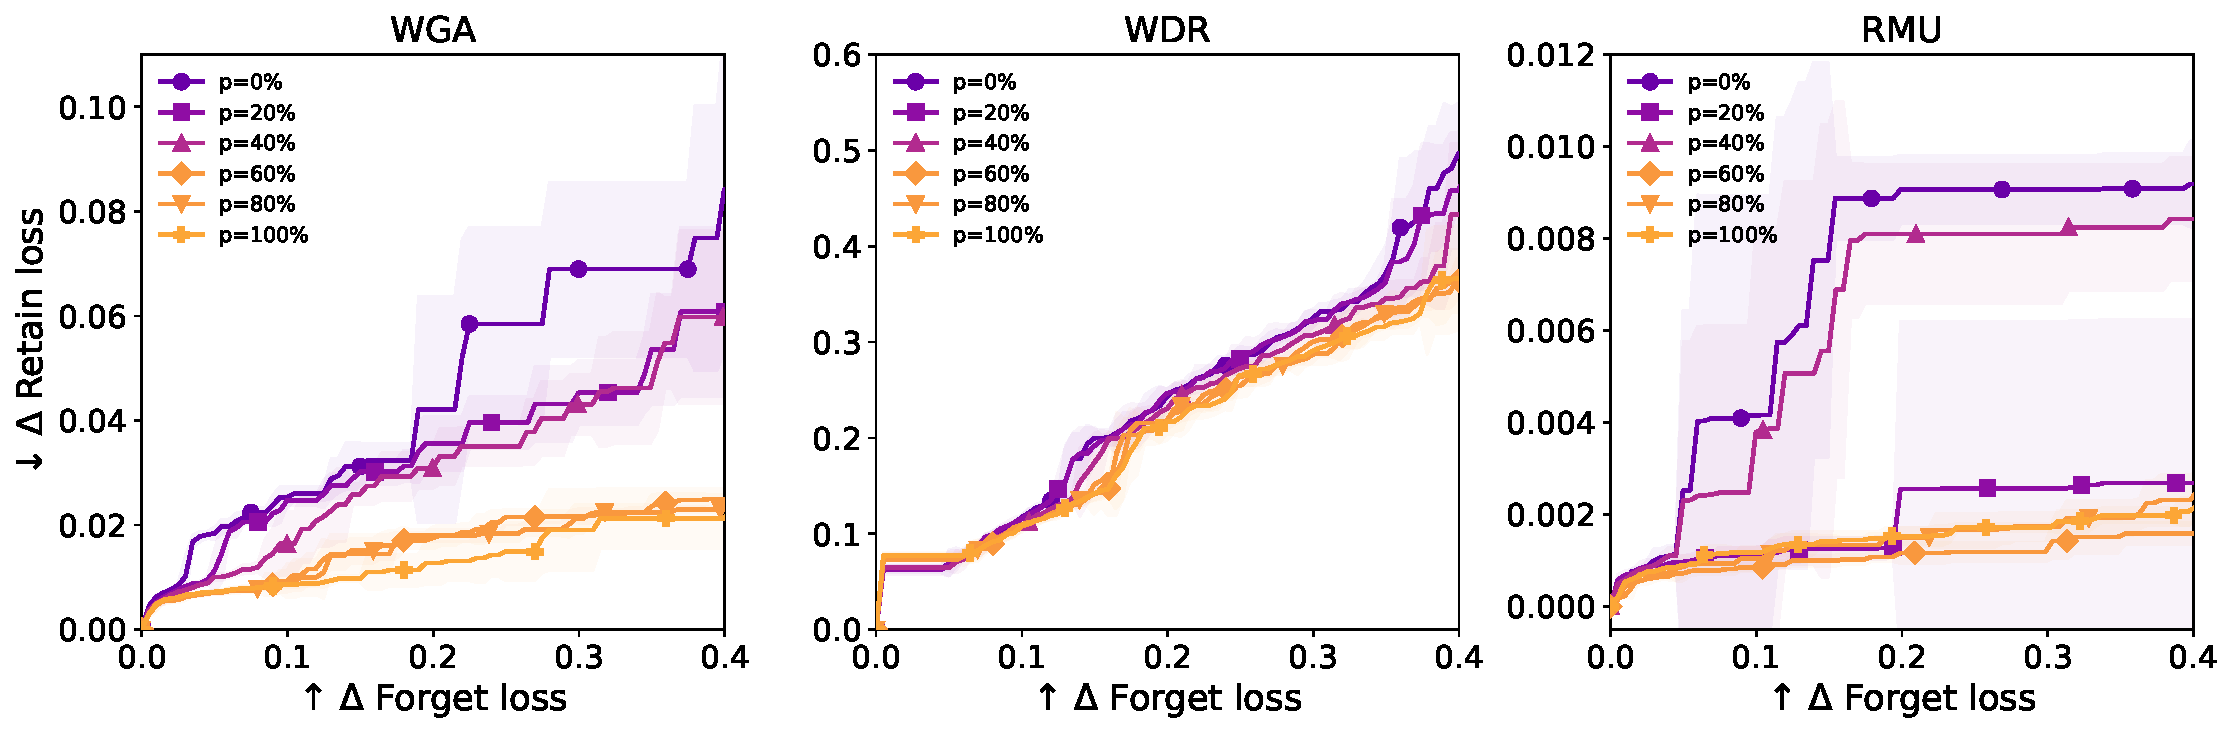
\includegraphics[width=\linewidth]{assets/wiki_retain_forget_tradeoff.pdf}
  \caption{The more disentangled the retain and forget sets are in a model, the better the retain-forget trade-offs achieved by unlearning. The plot shows retain-forget Pareto frontiers of three unlearning methods across six models with varying amounts of SGTM applied during training ($p$). Models are colored according to their Variance Entanglement Score (\cref{sec:entanglement}): the purple are less disentangled, the yellow are more disentangled. Each frontier is constructed over 4--6 hyperparameter configurations, shaded regions show $\pm 1$ standard error across 5 seeds. The axes are measured relative to each model's losses before unlearning.}
  \label{figure:unlearning}
\end{figure}

These results confirm the longstanding intuition that entanglement is a meaningful factor in unlearning difficulty, and show that even standard unlearning methods can benefit from operating on models with more separated internal representations.

\section{Experimental Setup}

Our experimental pipeline has two stages: first, we train a suite of models with varying degrees of knowledge entanglement using Selective Gradient Masking (SGTM) (\cref{sec:training}), and then we apply standard unlearning algorithms to each model and measure the resulting retain--forget trade-off (\cref{sec:unlearning}).

% ======================================================================
\subsection{Training a Spectrum of Disentangled Models with SGTM}
\label{sec:training}

For training disentangled models, we use SGTM~\citep{shilov2025datafilteringknowledgelocalization}, a recent method for training models so that pre-selected parameters are specialized to a target data domain. We closely follow the training setup in the original paper, including dataset, model architecture, the implementation of SGTM itself, and hyperparameters. \textbf{Our only modifications} are to reduce the number of evaluation examples, and to vary the fraction of training during which SGTM is active, producing six models that span a range of entanglement levels.

\paragraph{Data.}
Following the original paper, we train on English Wikipedia (approximately 3.7B tokens), using the same article-level topic labels derived from Wikipedia's \texttt{articletopic} classifier. We assign each training example to one of three categories that govern how it is treated during SGTM training:
%
\begin{itemize}[nosep,leftmargin=1.5em]
  \item $\mathcal{D}_\text{forget}$: all articles classified as STEM.Biology (${\sim}3.7\%$ of training tokens);
  \item $\mathcal{D}_\text{retain}$: a randomly sampled $10\%$ of the remaining (non-biology) articles, treated as confidently-labeled retain data;
  \item $\mathcal{D}_\text{unlabeled}$: the remaining $90\%$ of non-biology articles, for which no label is assumed.
\end{itemize}
%
For evaluation, we hold out a biology test set (used to measure forget loss) and a non-biology test set spanning all other topic categories (used to measure retain loss). To reduce evaluation cost during our hyperparameter sweeps, we subsample $20\%$ of each test set and report all metrics on this fixed subsample.

% --- Model ---

\paragraph{Model.}
We train a 254M-parameter GPT-Neo-style transformer with 16 layers, hidden dimension 1024, 32 attention heads, and MLP dimension 4096. We adopt all training hyperparameters from the original paper; see \cref{tab:training-hyperparams} in Appendix \ref{app:hyperparams} for the full configuration. In each transformer block, we designate a small subset of parameters as the \emph{forget subnetwork}:
%
\begin{itemize}[nosep,leftmargin=1.5em]
  \item $\theta_\text{forget}$: 1 attention head (out of 32) and 64 MLP hidden units (out of 4{,}096) per block;
  \item $\theta_\text{retain}$: all remaining parameters.
\end{itemize}
%
This designation is used during SGTM training (described next) to make $\theta_\text{forget}$ specialize on processing forget-domain data.

% --- SGTM ---

\paragraph{Training with SGTM.}
SGTM is a modification to the training procedure that applies different interventions to the forward and backward passes depending on which of the three data categories ($\mathcal{D}_\text{forget}$, $\mathcal{D}_\text{retain}$, $\mathcal{D}_\text{unlabeled}$) an example belongs to. The interventions are summarized in \cref{tab:interventions}

In the standard SGTM pipeline, these interventions are applied throughout training; our adaptation (described in the next paragraph) instead activates them for only a fraction of the training steps.

\begin{table}[h]
  \centering
  \small
  \begin{tabular}{@{}lccc@{}}
    \toprule
    \textbf{Data subset} & \textbf{Forward pass} & \textbf{Backward pass} & \textbf{Updated params} \\
    \midrule
    $\mathcal{D}_\text{forget}$ & --- & Zero $\nabla_{\theta_\text{retain}}$ & $\theta_\text{forget}$ only \\
    $\mathcal{D}_\text{unlabeled}$ & --- & --- & $\theta_\text{forget}$ and $\theta_\text{retain}$ \\
    $\mathcal{D}_\text{retain}$ & Set $\theta_\text{forget} = 0$ & --- & $\theta_\text{retain}$ only$^{\dagger}$ \\
    \bottomrule
  \end{tabular}
  \caption{Training interventions in SGTM, applied per-example based on its data category. ``---'' indicates standard (unmodified) behavior. $^{\dagger}$\,$\theta_\text{forget}$ receives no gradient because its activations are zeroed during the forward pass.}
  \label{tab:interventions}
\end{table}

For forget examples, gradients for $\theta_\text{retain}$ are zeroed after the backward pass, ensuring that forget-domain knowledge flows only into the designated forget subnetwork. For retain examples, $\theta_\text{forget}$ is zeroed during the forward pass, training the model to perform well on retain data even without the forget subnetwork. Unlabeled examples update all parameters via standard training.

% --- Our modification ---

\paragraph{Creating a spectrum of entanglement.}
To produce models with different degrees of disentanglement, we train six models with different amounts of SGTM exposure ($p$), ranging from $p=0\%$ to $p=100\%$. In a model with $p\%$ SGTM exposure, the first $(100{-}p)\%$ of training steps use standard training (no SGTM interventions), and the remaining $p\%$ apply full SGTM according to \cref{tab:interventions}. We train models with $p \in \{0, 20, 40, 60, 80, 100\}$, where $p{=}0$ is a fully standard model and $p{=}100$ applies SGTM during the entire training process (biology knowledge is strongly concentrated in $\theta_\text{forget}$). Intuitively, models with more SGTM exposure should exhibit greater separation of forget and retain knowledge in parameter space; we verify this in \cref{sec:entanglement} using several proxy metrics of entanglement from the literature.

Readers already familiar with SGTM should note that after training we do \emph{not} ablate $\theta_\text{forget}$. We use SGTM solely for the purpose of controlling entanglement, not for unlearning itself. We also note that applying SGTM stochastically---routing each forget example with some probability rather than front-loading standard training and then switching to full SGTM---would produce substantial disentanglement even at low routing probabilities, due to the \emph{absorption effect} described by~\citet{cloud2024gradientroutingmaskinggradients, shilov2025datafilteringknowledgelocalization}. Our phased scheme avoids this by cleanly separating the standard and SGTM portions of training, yielding a more controllable spectrum of entanglement levels.

% ======================================================================
\subsection{Measuring Retain--Forget Trade-off During Unlearning}
\label{sec:unlearning}

Given the six models, we apply three standard unlearning algorithms to each, aiming to remove the forget knowledge. The unlearning algorithm receives the full model with no information about how it was trained or where biology knowledge might be stored. Our interest is not in comparing methods against each other but rather in whether, \emph{within each method}, more disentangled models yield better retain--forget trade-offs. Full hyperparameter configurations for each method are given in \cref{tab:wga-hyperparams}--\ref{tab:rmu-hyperparams} in Appendix \ref{app:unlearning-hyperparams}.

In what follows, $\operatorname{CE}(\theta;\, \mathcal{D})$ denotes the mean per-token cross-entropy of model~$\theta$ on dataset~$\mathcal{D}$.

% --- WGA ---

\paragraph{Weighted Gradient Ascent (WGA).}
WGA combines gradient ascent on the forget set with gradient descent on the retain set~\citep{wang2025rethinking}, minimizing:
%
\begin{equation*}
  \mathcal{L}_\text{WGA}(\theta)
  = \operatorname{CE}(\theta;\, \mathcal{D}_\text{retain})
  - \lambda_\text{WGA}\, \operatorname{CE}_\text{WGA}(\theta;\, \mathcal{D}_\text{forget}),
  \quad \lambda_\text{WGA} > 0
\end{equation*}
%
where $\operatorname{CE}_\text{WGA}$ is a reweighted cross-entropy that scales each token's log-probability loss by $[p_\theta(x_t \mid x_{<t})]^\alpha$ (with $\alpha$ set to $0.1$ in our experiments). This upweights tokens the model predicts confidently, so that gradient ascent targets the most well-learned predictions first. During training, on each step, the method draws one batch from each split.

% --- WDR ---

\paragraph{Weight Divergence Regularization (WDR).}
Following~\citet{siddiqui2025dormant}, we fine-tune on the retain set while simultaneously maximizing the $L_2$ distance between the current parameters $\theta$ and the original pretrained parameters $\theta_0$:
%
\begin{equation*}
  \mathcal{L}_\text{WDR}(\theta)
  = \operatorname{CE}(\theta;\, \mathcal{D}_\text{retain})
  - \lambda_\text{WDR}\, \sqrt{\frac{1}{|\theta|}\sum_i (\theta_i - \theta_{0,i})^2},
  \quad \lambda_\text{WDR} > 0
\end{equation*}
%
This encourages the unlearned model to move far from the pretrained model in weight space, which~\citet{siddiqui2025dormant} show correlates with improved tamper-resistance against relearning attacks.

% --- RMU ---

\paragraph{Representation Misdirection for Unlearning (RMU).}
RMU~\cite{li2024wmdp} modifies intermediate representations at a designated layer so that, on forget examples, activations are steered toward random target directions, while on retain examples, activations are anchored to their pretrained values. Only the MLP weights at the target layers are updated.

% --- Sweep, frontier ---

\paragraph{Hyperparameter sweep and the retain--forget Pareto frontier.}
For each method, we sweep over 4--6 hyperparameter configurations (varying learning rate and the method-specific coefficient). We run each configuration with 5 random seeds for a method-specific number of optimizer steps, with early stopping when the forget loss exceeds the loss of a model trained with no biology data plus a small buffer ($\ell = 3.33$).\footnote{Beyond this point, further increasing the forget loss reflects model degradation rather than meaningful knowledge removal.} For each model and method, we construct a Pareto frontier over all the hyperparameter configurations, with confidence intervals derived from the per-seed variation. The full configurations are reported in Appendix~\ref{app:unlearning-hyperparams}.

\section{Results}

\subsection{Models trained with more SGTM exposure are more disentangled}
\label{sec:entanglement}

Before evaluating unlearning, we verify that our phased training scheme (\cref{sec:training}) produces models with meaningfully different levels of entanglement. There is no single agreed-upon definition of entanglement, so following~\citet{tang2026logitslatentscontrastiverepresentation} we adopt three complementary proxy metrics from the literature. All three metrics are described below.

In \cref{figure:disentanglement}, we normalize each metric to $[0, 1]$ and plot how it varies with SGTM exposure~$p$. Across all three metrics, models with higher SGTM exposure ($p \geq 60\%$) show substantially greater retain--forget disentanglement than models with lower exposure ($p \leq 40\%$). As a control, we also compute each metric between the retain set and an the adjacent set, whose relationship to the retain set should not change with SGTM exposure. We find that retain--adjacent separation remains roughly constant across all values of~$p$, confirming that the observed trend reflects genuine localization of biology knowledge rather than a general distortion of the representation space.

\begin{figure}[t]
  \centering
  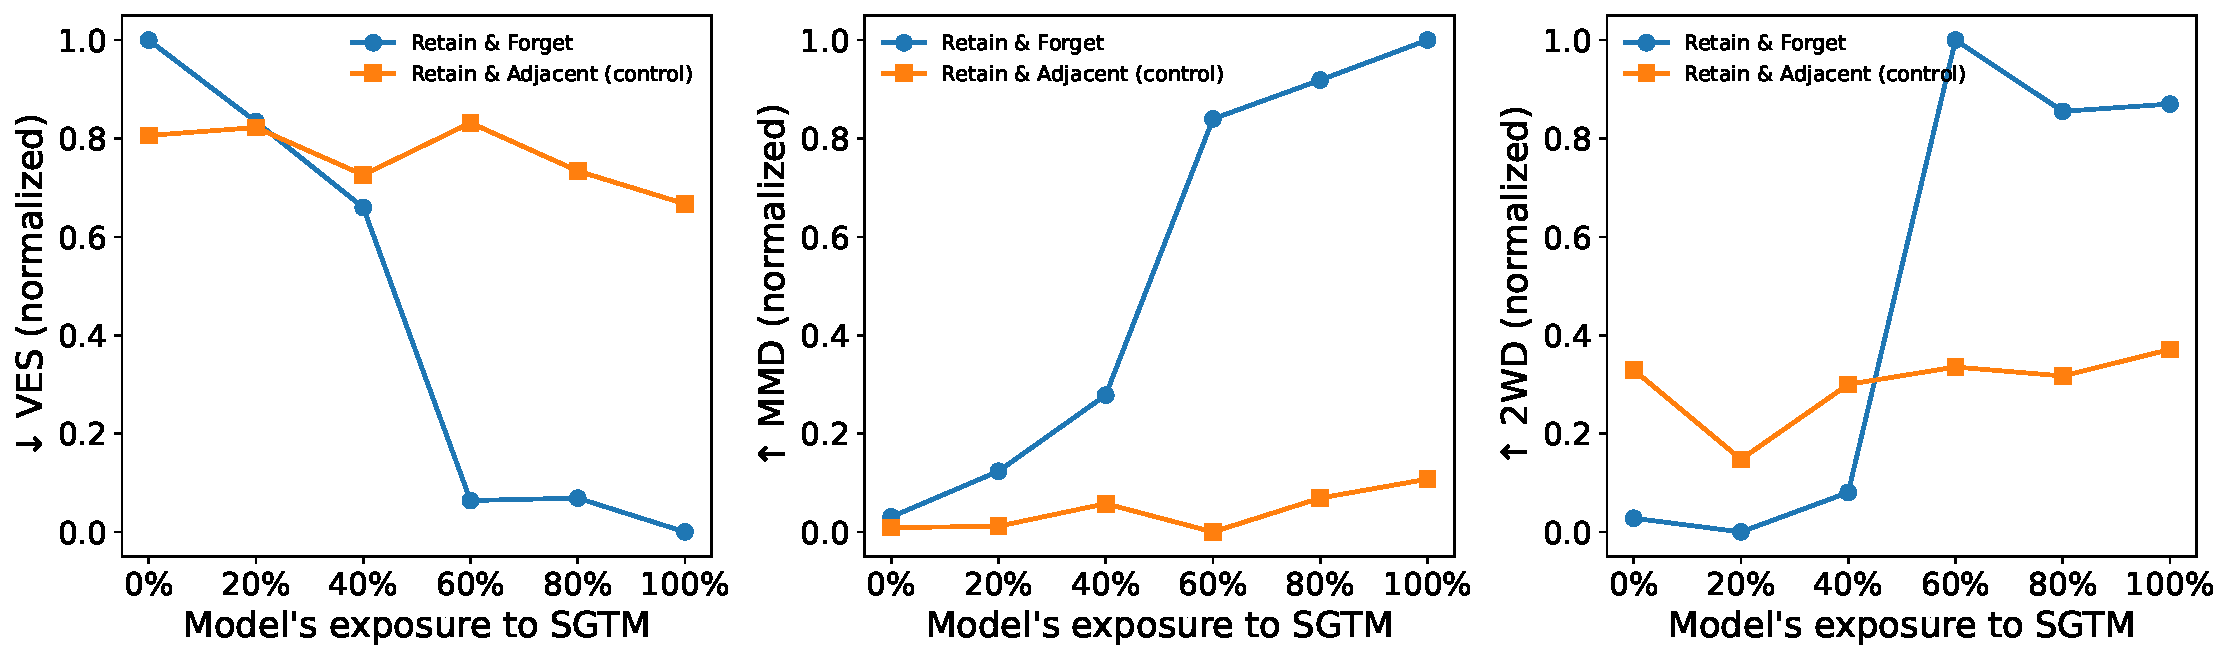
\includegraphics[width=\linewidth]{assets/wiki_entanglement_normalized.pdf}
  \caption{Three proxy metrics of retain--forget disentanglement as a function of model's exposure to SGTM exposure, each normalized to $[0, 1]$, with retain--adjacent as control. All three metrics show a sharp increase in retain--forget disentanglement between $40\%$ and $60\%$, while retain--adjacent disentanglement remains roughly flat, confirming that SGTM selectively disentangles forget knowledge. \textbf{Left:} Variance Entanglement Score (lower = more disentangled). \textbf{Center:} Multi-kernel MMD (higher = more disentangled). \textbf{Right:} 2-Wasserstein distance (higher = more disentangled).}
  \label{figure:disentanglement}
\end{figure}

We now briefly describe each metric.

\begin{itemize}[leftmargin=1.5em]
  \item \textbf{Variance Entanglement Score (VES)}~\cite{zhao2024what} compares within-group spread to between-group separation. Let $\phi(x) \in \mathbb{R}^d$ denote the model's hidden representation of input~$x$ at a chosen intermediate layer, then
    %
    \begin{equation*}
      \mathrm{VES} = \frac{
        \frac{1}{|\mathcal{R}|}\sum_{i \in \mathcal{R}} \|\phi(x_i) - \mu_{\mathcal{R}}\|^2
        + \frac{1}{|\mathcal{F}|}\sum_{j \in \mathcal{F}} \|\phi(x_j) - \mu_{\mathcal{F}}\|^2
      }{
        \|\mu_{\mathcal{R}} - \mu\|^2 + \|\mu_{\mathcal{F}} - \mu\|^2
      }
    \end{equation*}
    %
    where $\mu_{\mathcal{R}}, \mu_{\mathcal{F}}$ are the mean representations of the retain and forget sets and $\mu$ is the overall mean. Lower VES indicates more disentanglement between the two groups.

  \item \textbf{Maximum Mean Discrepancy (MMD)}~\cite{JMLR:v13:gretton12a} is a nonparametric two-sample statistic that tests whether two sets of representations come from the same distribution. It maps both sets into a reproducing kernel Hilbert space and measures the distance between their mean embeddings. We use a multi-kernel variant that sums six Gaussian kernels at bandwidths $\sigma \in \{0.1, 0.25, 0.5, 1.0, 2.0, 4.0\}$, making the statistic sensitive to distributional differences at multiple scales. Higher MMD indicates more disentanglement.

  \item \textbf{2-Wasserstein distance (2WD)} is an optimal-transport metric that measures the minimum cost of transforming one distribution into another. Higher distance indicates greater disentanglement.
\end{itemize}

\subsection{More disentangled models achieve better retain--forget trade-offs}
\label{sec:results}

We now evaluate whether the degree of disentanglement affects the retain--forget trade-off during unlearning.
We focus on the \emph{change} in forget and retain loss during unlearning relative to each model's own pre-unlearning baseline instead of the absolute losses because the six models have different pre-unlearning losses.
For each of the six models, we run the three unlearning methods described in \cref{sec:unlearning} across all hyperparameter configurations and seeds, and construct Pareto frontiers in the $(\Delta\ell_\text{retain},\, \Delta\ell_\text{forget})$ plane.

The main finding is that more disentangled models consistently achieve better retain--forget trade-offs, though we cannot fully disentangle its effect from other correlated properties of the training trajectory. \Cref{figure:unlearning} shows the results.

In WGA, the effect is clearest. At a fixed forget-loss increase of $\Delta\ell_\text{forget} = 0.4$, the most disentangled model ($p{=}100\%$) incurs roughly $4\times$ lower retain cost than the most entangled one ($p{=}0\%$). The Pareto frontiers separate into two clusters, according to the entanglement scores observed in \cref{sec:entanglement}: models with low disentanglement ($p \leq 40\%$) form one cluster, and models with high disentanglement ($p \geq 60\%$) form another.

WDR shows the same directional trend, though the frontiers are closer together and the confidence intervals overlap. At the same $\Delta\ell_\text{forget} = 0.4$ point, the $p=100\%$ model incurs roughly $1.3\times$ lower retain cost than at the $p=0\%$ model.

In RMU, the retain-loss scale is two orders of magnitude smaller than in WDR, reflecting RMU's minimal impact on retain performance overall. Even at this scale, the effect persists: the $p=100\%$ model incurs roughly $4\times$ lower retain cost than the $p=0\%$ model at the same $\Delta\ell_\text{forget} = 0.4$ point, and the low disentanglement models incur consistently higher retain costs than the high disentanglement ones. A notable exception is the $p=20\%$ model, which performs comparably to $p=60\%$, $p=80\%$, and $p=100\%$.

It's important to note that the choice of unlearning method has a far larger effect on the retain--forget trade-off than the degree of entanglement. Disentanglement modulates the frontier within a method, but the method determines the operating regime. Our finding should be read not as ``disentangle your models before unlearning,'' but as evidence that unlearning difficulty depends on the degree of knowledge entanglement in the model.

\section*{Acknowledgments}

\bibliography{iclr2026_conference}
\bibliographystyle{iclr2026_conference}

\appendix

\section{Training Hyperparameters} \label{app:hyperparams}

See \cref{tab:training-hyperparams} for the full training hyperparameters.

\begin{table}[h]
  \centering
  \small
  \begin{tabular}{@{}ll@{}}
    \toprule
    \textbf{Hyperparameter} & \textbf{Value} \\
    \midrule
    Parameters & 254M \\
    Layers & 16 \\
    Hidden dimension ($d$) & 1024 \\
    Attention heads ($h$) & 32 \\
    MLP dimension ($d_\text{MLP}$) & 4096 \\
    Context size & 1024 \\
    Vocabulary size & 50{,}257 \\
    Tied embeddings & True \\
    Tokenizer & GPT-2 \\
    \midrule
    Optimizer & AdamW \\
    Learning rate & $6 \times 10^{-4}$ \\
    LR schedule & Cosine annealing with warmup \\
    Warmup steps & 1{,}000 \\
    Total training steps & 9{,}689 \\
    Batch size & 16 \\
    Weight decay & 0.1 \\
    $\beta_1$ & 0.9 \\
    $\beta_2$ & 0.95 \\
    \midrule
    Forget MLP dim ($d_\text{forget}$) & 64 \\
    Forget attention heads ($h_\text{forget}$) & 1 \\
    Confident retain fraction & 10\% \\
    Mask embeddings & True \\
    \bottomrule
  \end{tabular}
  \caption{Training hyperparameters, following~\citet{shilov2025datafilteringknowledgelocalization}.}
  \label{tab:training-hyperparams}
\end{table}

\section{Unlearning Hyperparameters} \label{app:unlearning-hyperparams}

All unlearning methods use the AdamW optimizer with no weight decay, evaluate every 5 steps on a $20\%$ subsample of each test set, and are run for a maximum of 50 steps. Each configuration is run with 5 seeds (42--46).

\begin{table}[h]
  \centering
  \small
  \begin{tabular}{@{}ll@{}}
    \toprule
    \textbf{Hyperparameter} & \textbf{Value} \\
    \midrule
    \multicolumn{2}{@{}l}{\textit{Fixed}} \\
    Total steps & 50 \\
    Eval every & 5 steps \\
    WGA $\alpha$ & 0.1 \\
    Retain loss coefficient & 1.0 \\
    \midrule
    \multicolumn{2}{@{}l}{\textit{Swept}} \\
    Learning rate & $\{1.25 \times 10^{-5},\; 2.5 \times 10^{-5},\; 5 \times 10^{-5}\}$ \\
    Forget loss coefficient ($\lambda_\text{f}$) & $\{0.128,\; 0.32\}$ \\
    \bottomrule
  \end{tabular}
  \caption{WGA hyperparameters (6 configurations).}
  \label{tab:wga-hyperparams}
\end{table}

\begin{table}[h]
  \centering
  \small
  \begin{tabular}{@{}ll@{}}
    \toprule
    \textbf{Hyperparameter} & \textbf{Value} \\
    \midrule
    \multicolumn{2}{@{}l}{\textit{Fixed}} \\
    Total steps & 100 \\
    Eval every & 10 steps \\
    Retain loss coefficient & 1.0 \\
    \midrule
    \multicolumn{2}{@{}l}{\textit{Swept}} \\
    Learning rate & $\{10^{-4},\; 2 \times 10^{-4},\; 4 \times 10^{-4}\}$ \\
    Divergence coefficient ($\lambda_\text{d}$) & $\{3,\; 30\}$ \\
    \bottomrule
  \end{tabular}
  \caption{WDR hyperparameters (6 configurations).}
  \label{tab:wdr-hyperparams}
\end{table}

\begin{table}[h]
  \centering
  \small
  \begin{tabular}{@{}ll@{}}
    \toprule
    \textbf{Hyperparameter} & \textbf{Value} \\
    \midrule
    \multicolumn{2}{@{}l}{\textit{Fixed}} \\
    Total steps & 100 \\
    Eval every & 5 steps \\
    Steering coefficient & 20 \\
    Retain anchoring coefficient ($\alpha$) & 100 \\
    Target layer & 7 \\
    Updated layers & 5, 6, 7 \\
    Updated parameters & MLP weights and biases \\
    Max gradient norm & 1.0 \\
    Early stopping min steps & 20 \\
    \midrule
    \multicolumn{2}{@{}l}{\textit{Swept}} \\
    Learning rate & $\{1.25 \times 10^{-5},\; 10^{-4},\; 8 \times 10^{-4},\; 6.4 \times 10^{-3}\}$ \\
    \bottomrule
  \end{tabular}
  \caption{RMU hyperparameters (4 configurations).}
  \label{tab:rmu-hyperparams}
\end{table}

\end{document}
